


%\section{Atuador}

%O motor elétrico é um dos dispositivos conversores de energia mais utilizados nos diversos meios tecnológicos, estando presentes largamente na indústria, em equipamentos eletrodomésticos, eletrônicos, automóveis, smarthphones, e uma variedade enorme de aplicações. 

%Os motores elétricos podem ser divididos em dois grandes grupos, em função do tipo de alimentação que utilizam, e são eles motores de corrente alternada, cuja velocidade pode ser controlada pela mudança da frequência e motores de corrente contínua, que basta alterar o nível de tensão para haver uma variação da velocidade, e no caso de motores de pequeno porte, são mais utilizados pela facilidade do seu controle. 

%O motor de corrente contínua (motor CC) é composto por uma parte fixa e outra móvel, denominadas respectivamente de Estator e Rotor. Seu princípio de funcionamento basicamente acontece pela relação de interação entre as forças eletromagnéticas. Uma bobina de fio é atravessada por um campo magnético gerado por ímãs fixos. Ao aplicar uma corrente elétrica na bobina, esta gera um campo elétrico que interage com o campo magnético gerando uma força de rotação, ou Torque, que faz o eixo girar. Quando a bobina, que forma o eixo de rotação se desloca até um determinado limite, seus terminais comutam e trocam de polaridade, mantendo os polos de interação sempre gerando a força de torção no eixo. O elemento que faz a troca de polaridade na bobina é denominado comutador.

%A velocidade de rotação do eixo depende da intensidade do campo elétrico gerado pela bobina e que interage com o campo magnetico gerada pelos ímãs fixos, assim, quanto maior for o campo gerado maior será a velocidade, e a intensidade do campo elétrico depende da intensidade de corrente que circula pela bobina, e esta depende da tensão aplicada aos teminais. Logo, alterando a tensão aplicada, altera-se a corrente, por consequência o campo elétrico e também a velocidade de rotação do motor.

%A Figura  \ref{fig:motorDC} mostra o motor CC utilizado no estudo mostrado neste trabalho, sendo um motor de baixa potência e baixo torque, mas de alta velocidade. 


%\begin{figure}[!htb]
%\center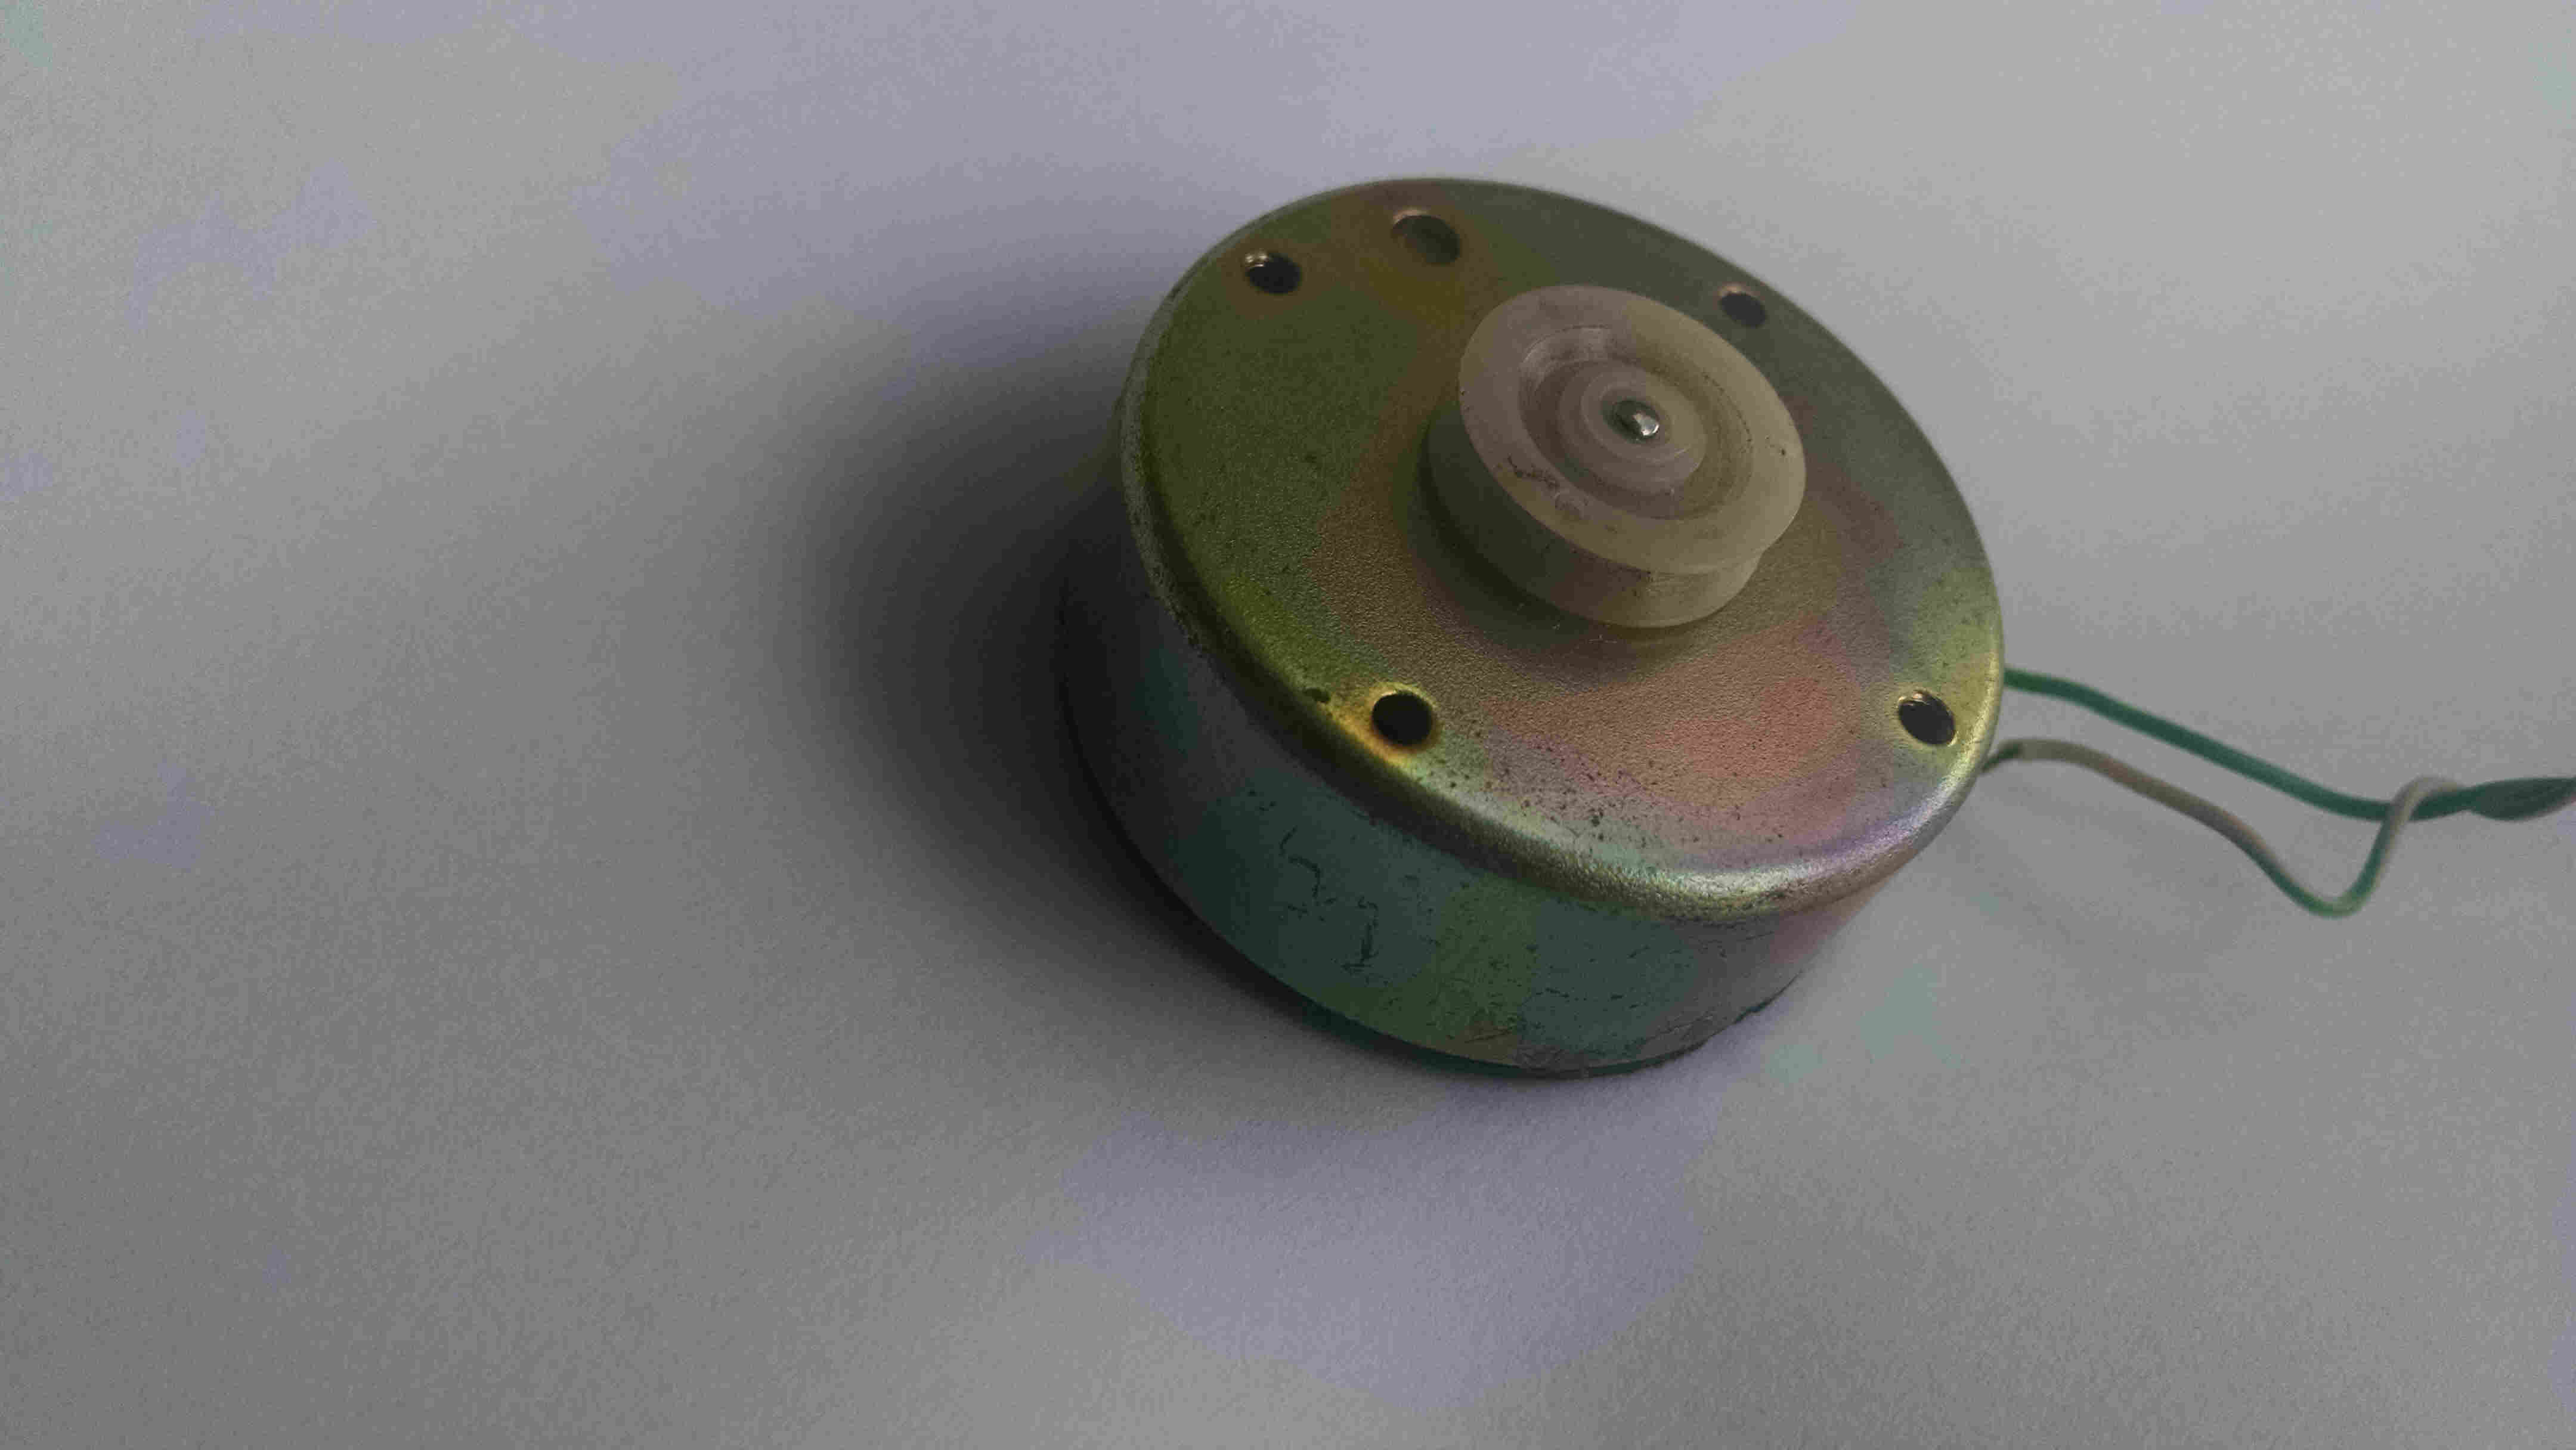
\includegraphics[scale=0.1, angle=0, clip=true, trim=1500 500 400 200]{./imagens/motorDC.jpg}
%\caption{Motor DC}
%\label{fig:motorDC}
%\end{figure}

%Para alimentação do motor, assim como do restante do sistema foi utilizada uma fonte chaveada de saída 12Vcc.


%O motor foi fixado a uma base de plástico com um furo contendo a medida de seu diâmetro, de forma a não haver folga e garantir uma estabilidade do motor sobre a superfície de repouso do sistema.

%Para gerar alguma carga, foi utilizado um CD acoplado ao eixo do motor, de forma centralizada e foi utilizada uma etiqueta de plástico presa na borda do CD para formar um ponto de leitura pelo sensor óptico, como se vê na Figura \ref{fig:discoSensor}.

%\section{Sensor}

%Para a leitura de velocidade foi utilizado um conjunto de sensor óptico para reconhecer cada giro do disco, e poder mensurar a velocidade de rotação do motor.

%A Figura \ref{fig:discoSensorGeral} mostra uma visão geral do sistema montado, utilizando o motor e o sensor posicionados de forma a serem feitas as experiências e testes pertinentes ao estudo.

%\begin{figure}[!htb]
%\center

%\subfloat[]{
%	\label{fig:discoSensor}
%	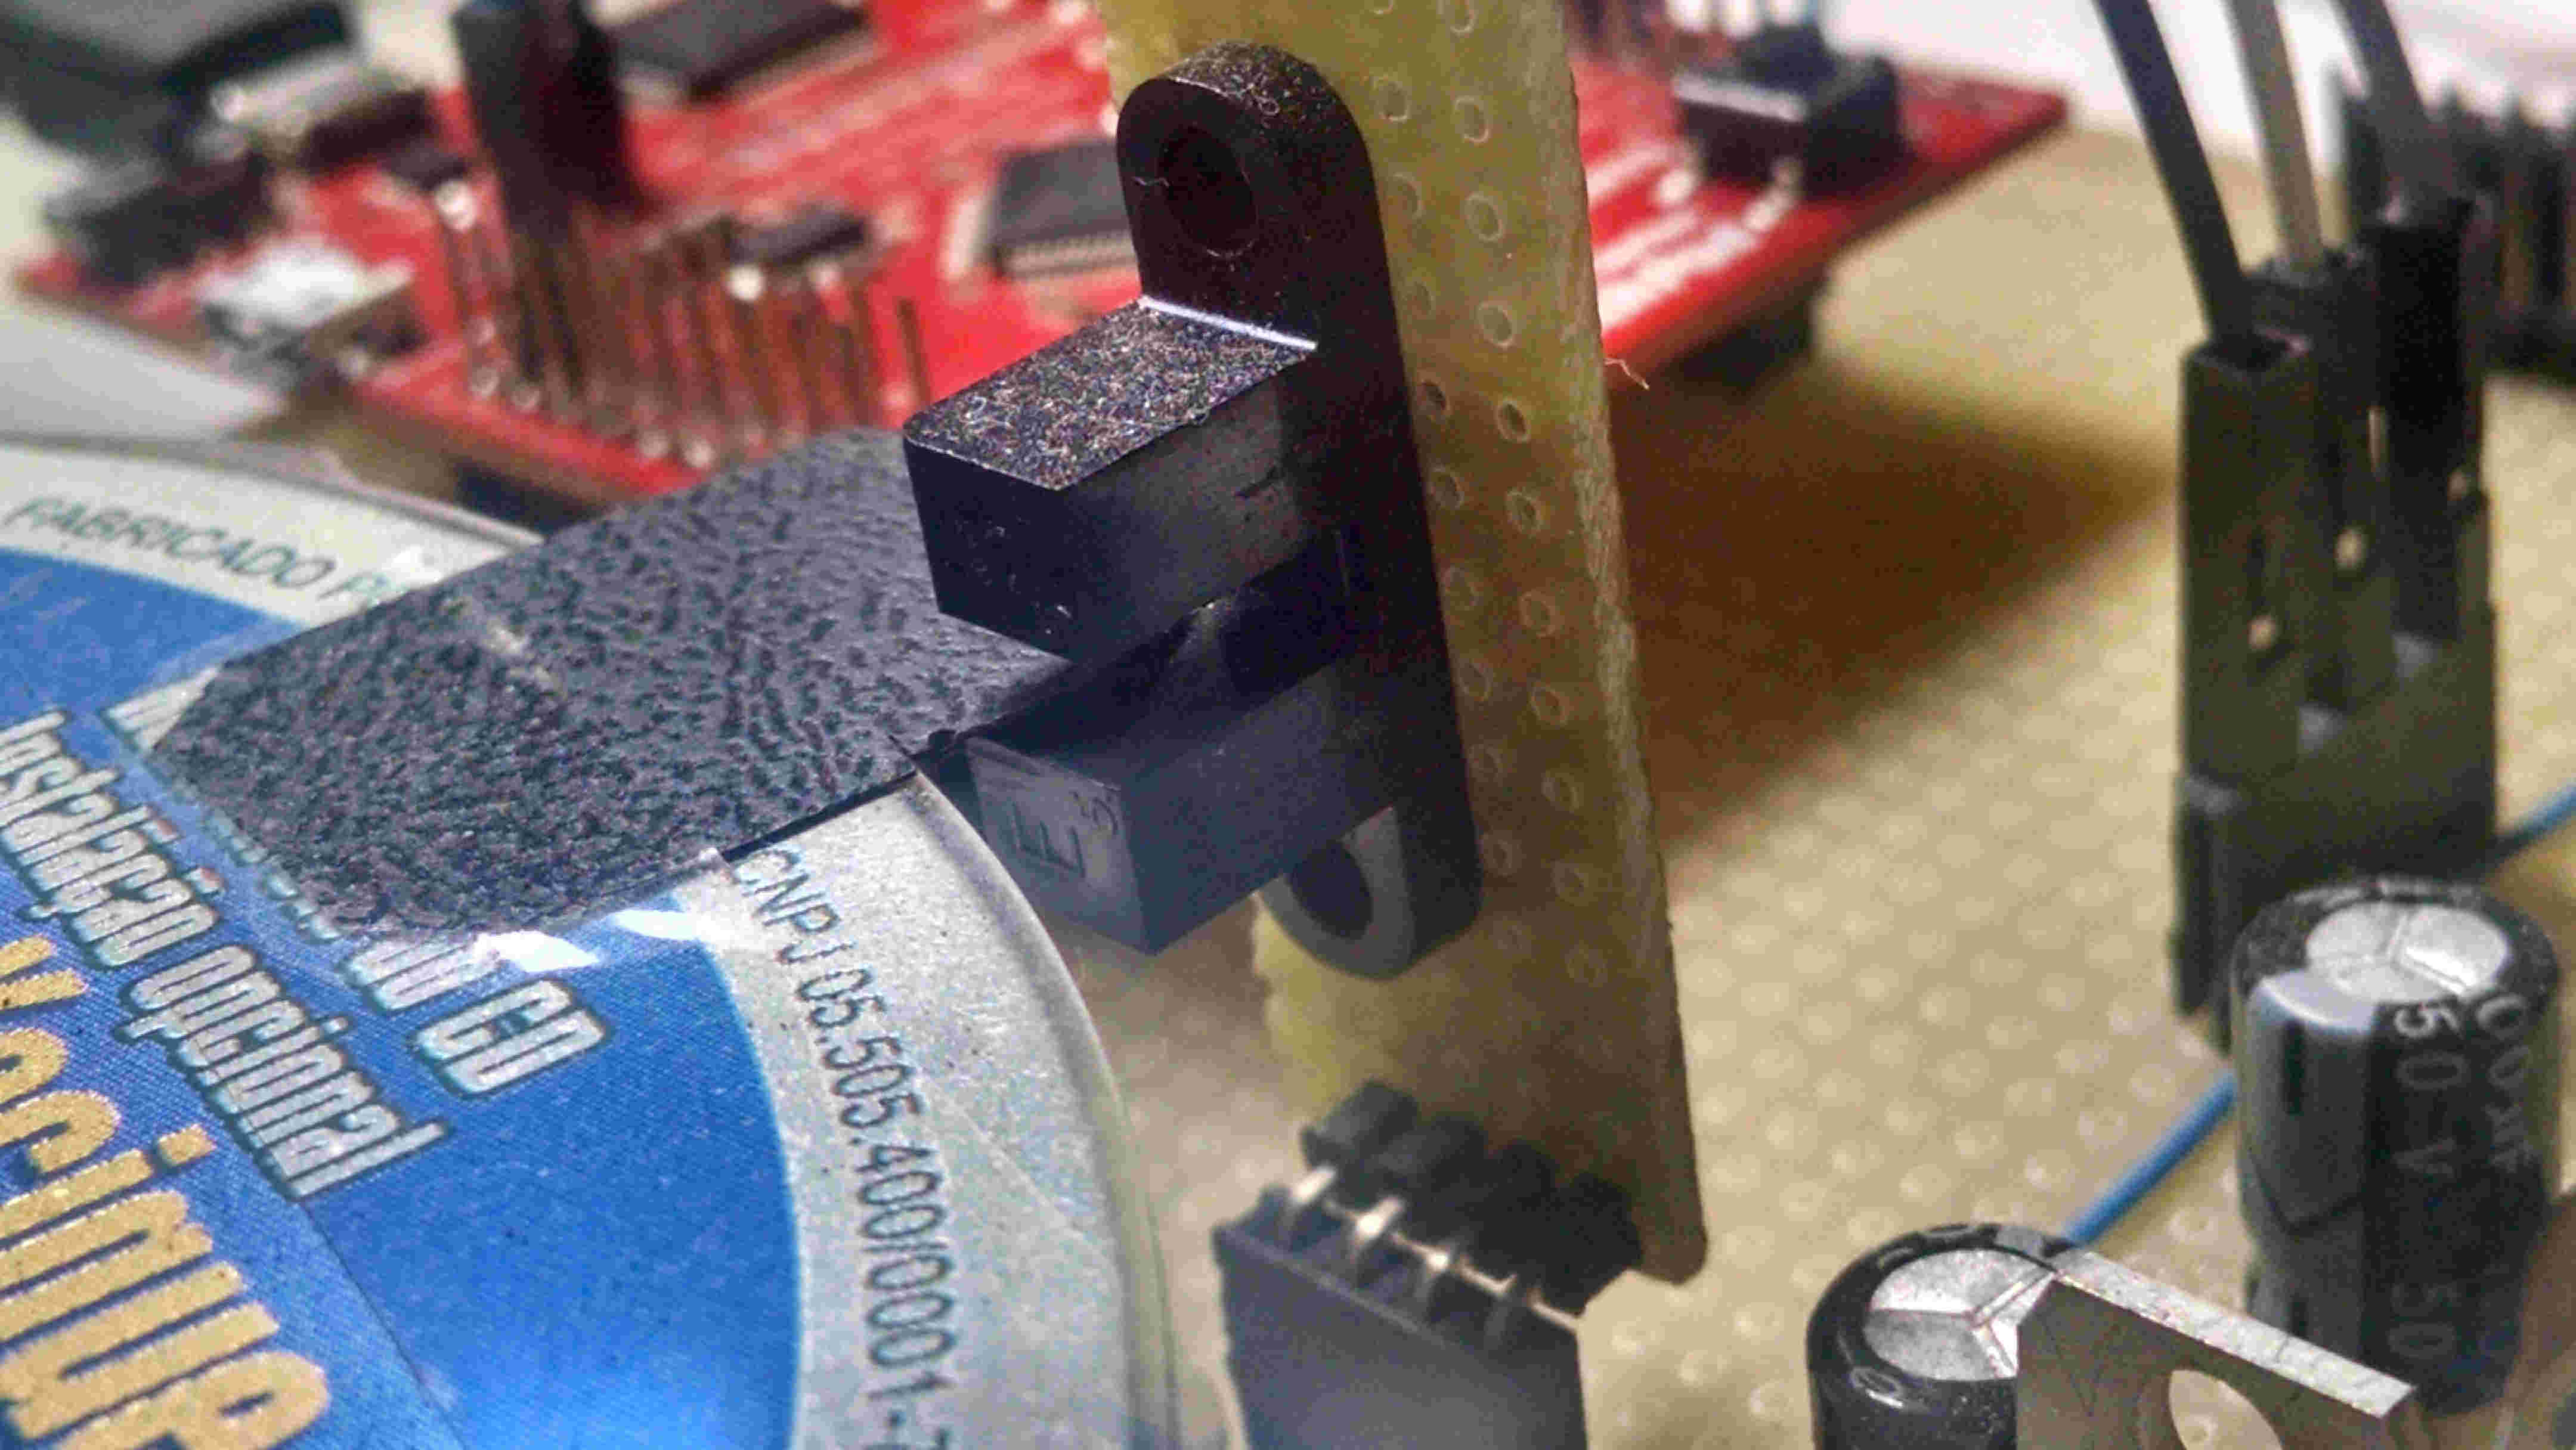
\includegraphics[scale=0.07, angle=0, clip=true, trim=300 200 1200 200]{./imagens/discoSensor.jpg}
%	}
%\subfloat[]{ 
%	\label{fig:discoSensorGeral} 
%	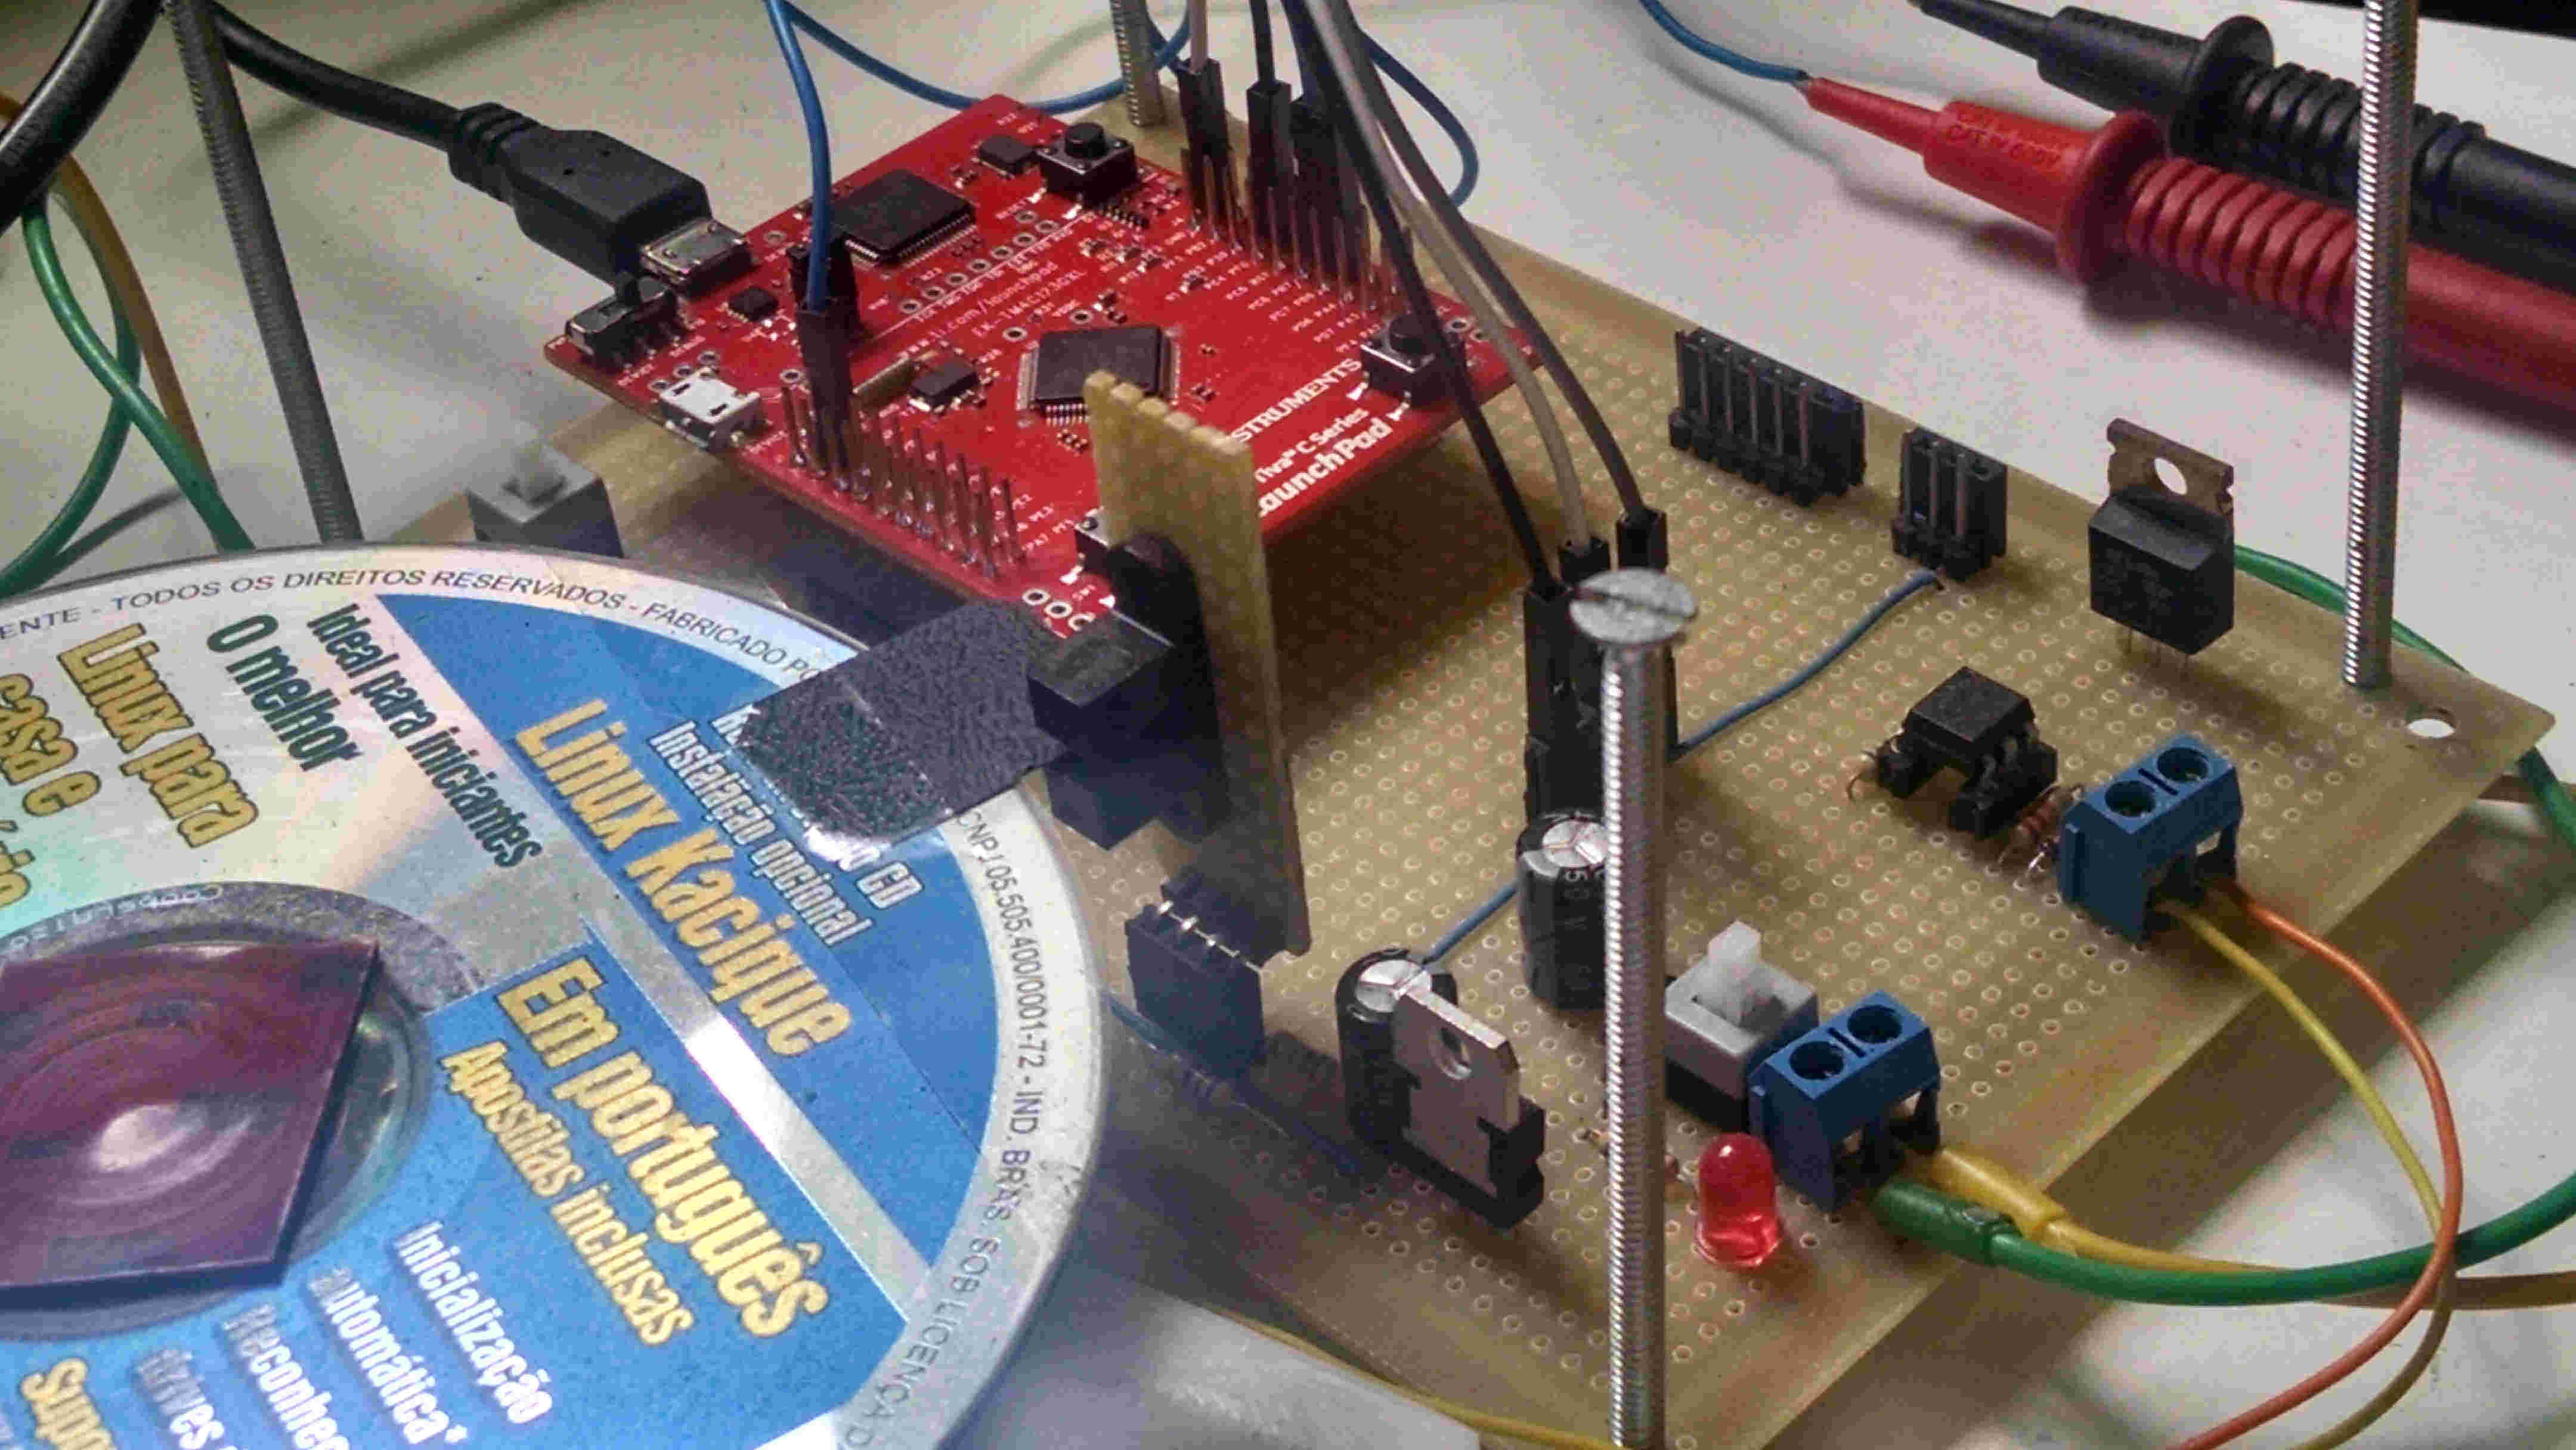
\includegraphics[scale=0.07, angle=0, clip=true, trim=300 200 400 200]{./imagens/discoSensorGeral.jpg} 
%	}

%\caption{Visão geral do sistema }
%\end{figure}





%\section{Drive}

%Para controlar a velocidade do motor cc, é necessário alterar a tensão aplicada nele, e a técnica mais comum é a Modulação por Largura de Pulso (do inglês: \emph{Pulse Width Modulation - PWM}, que consiste em chavear a alimentação a uma frequência fixa mas modulando, ou seja, alterando a largura dos pulsos, de forma que a tensão média aplicada possa ser controlada e o motor tenha uma alimentação que varia de zero até o valor da fonte para os respectivos valores de PWM.

%\begin{figure}[!htb]
%\center\includegraphics[scale=0.1, angle=0, clip=true, trim=0 0 0 0]{./imagens/drive.jpg}
%\caption{Drive}
%\label{fig:drive}
%\end{figure}

%Como elemento de acionamento do motor foi utilizado um transistor tipo MOS e um optoacoplador para isolar o acionamento do motor do controlador.

%\section{Controlador}

%Para o estudo proposto foi utilizado uma placa de desenvolvimento da Texas Instruments de modelo Tiva$^{TM}$ TM4C123GH6PM. A sua escolha deveu-se ao fato de que ela possui um controlador de 32bits, núcleo ARM.

%\begin{itemize}
%\item Núcleo (Core): ARM Cortex-M4F;
%\item Performance: 80 MHz em operação;
%\item Flash: 256 KB;
%\item Interface de comunicação:
%	\begin{itemize}
%	\item  Universal Asyncrhronous Receivers/Transmitter(UART);
%  	\item Inter-Integrated Circuit (I$^2$C);
%	\item Universal Serial Bus (USB);
%	\end{itemize}
%\item Periféricos:
%	\begin{itemize}
%	\item General-Purpose Input/Output (GPIO);
%	\item General-Purpose Timer (GPTM);
%	\item Módulo PWM: Pulse Width Modulator (PWM);
%	\end{itemize}
%\end{itemize}


%\begin{figure}[!htb]
%\center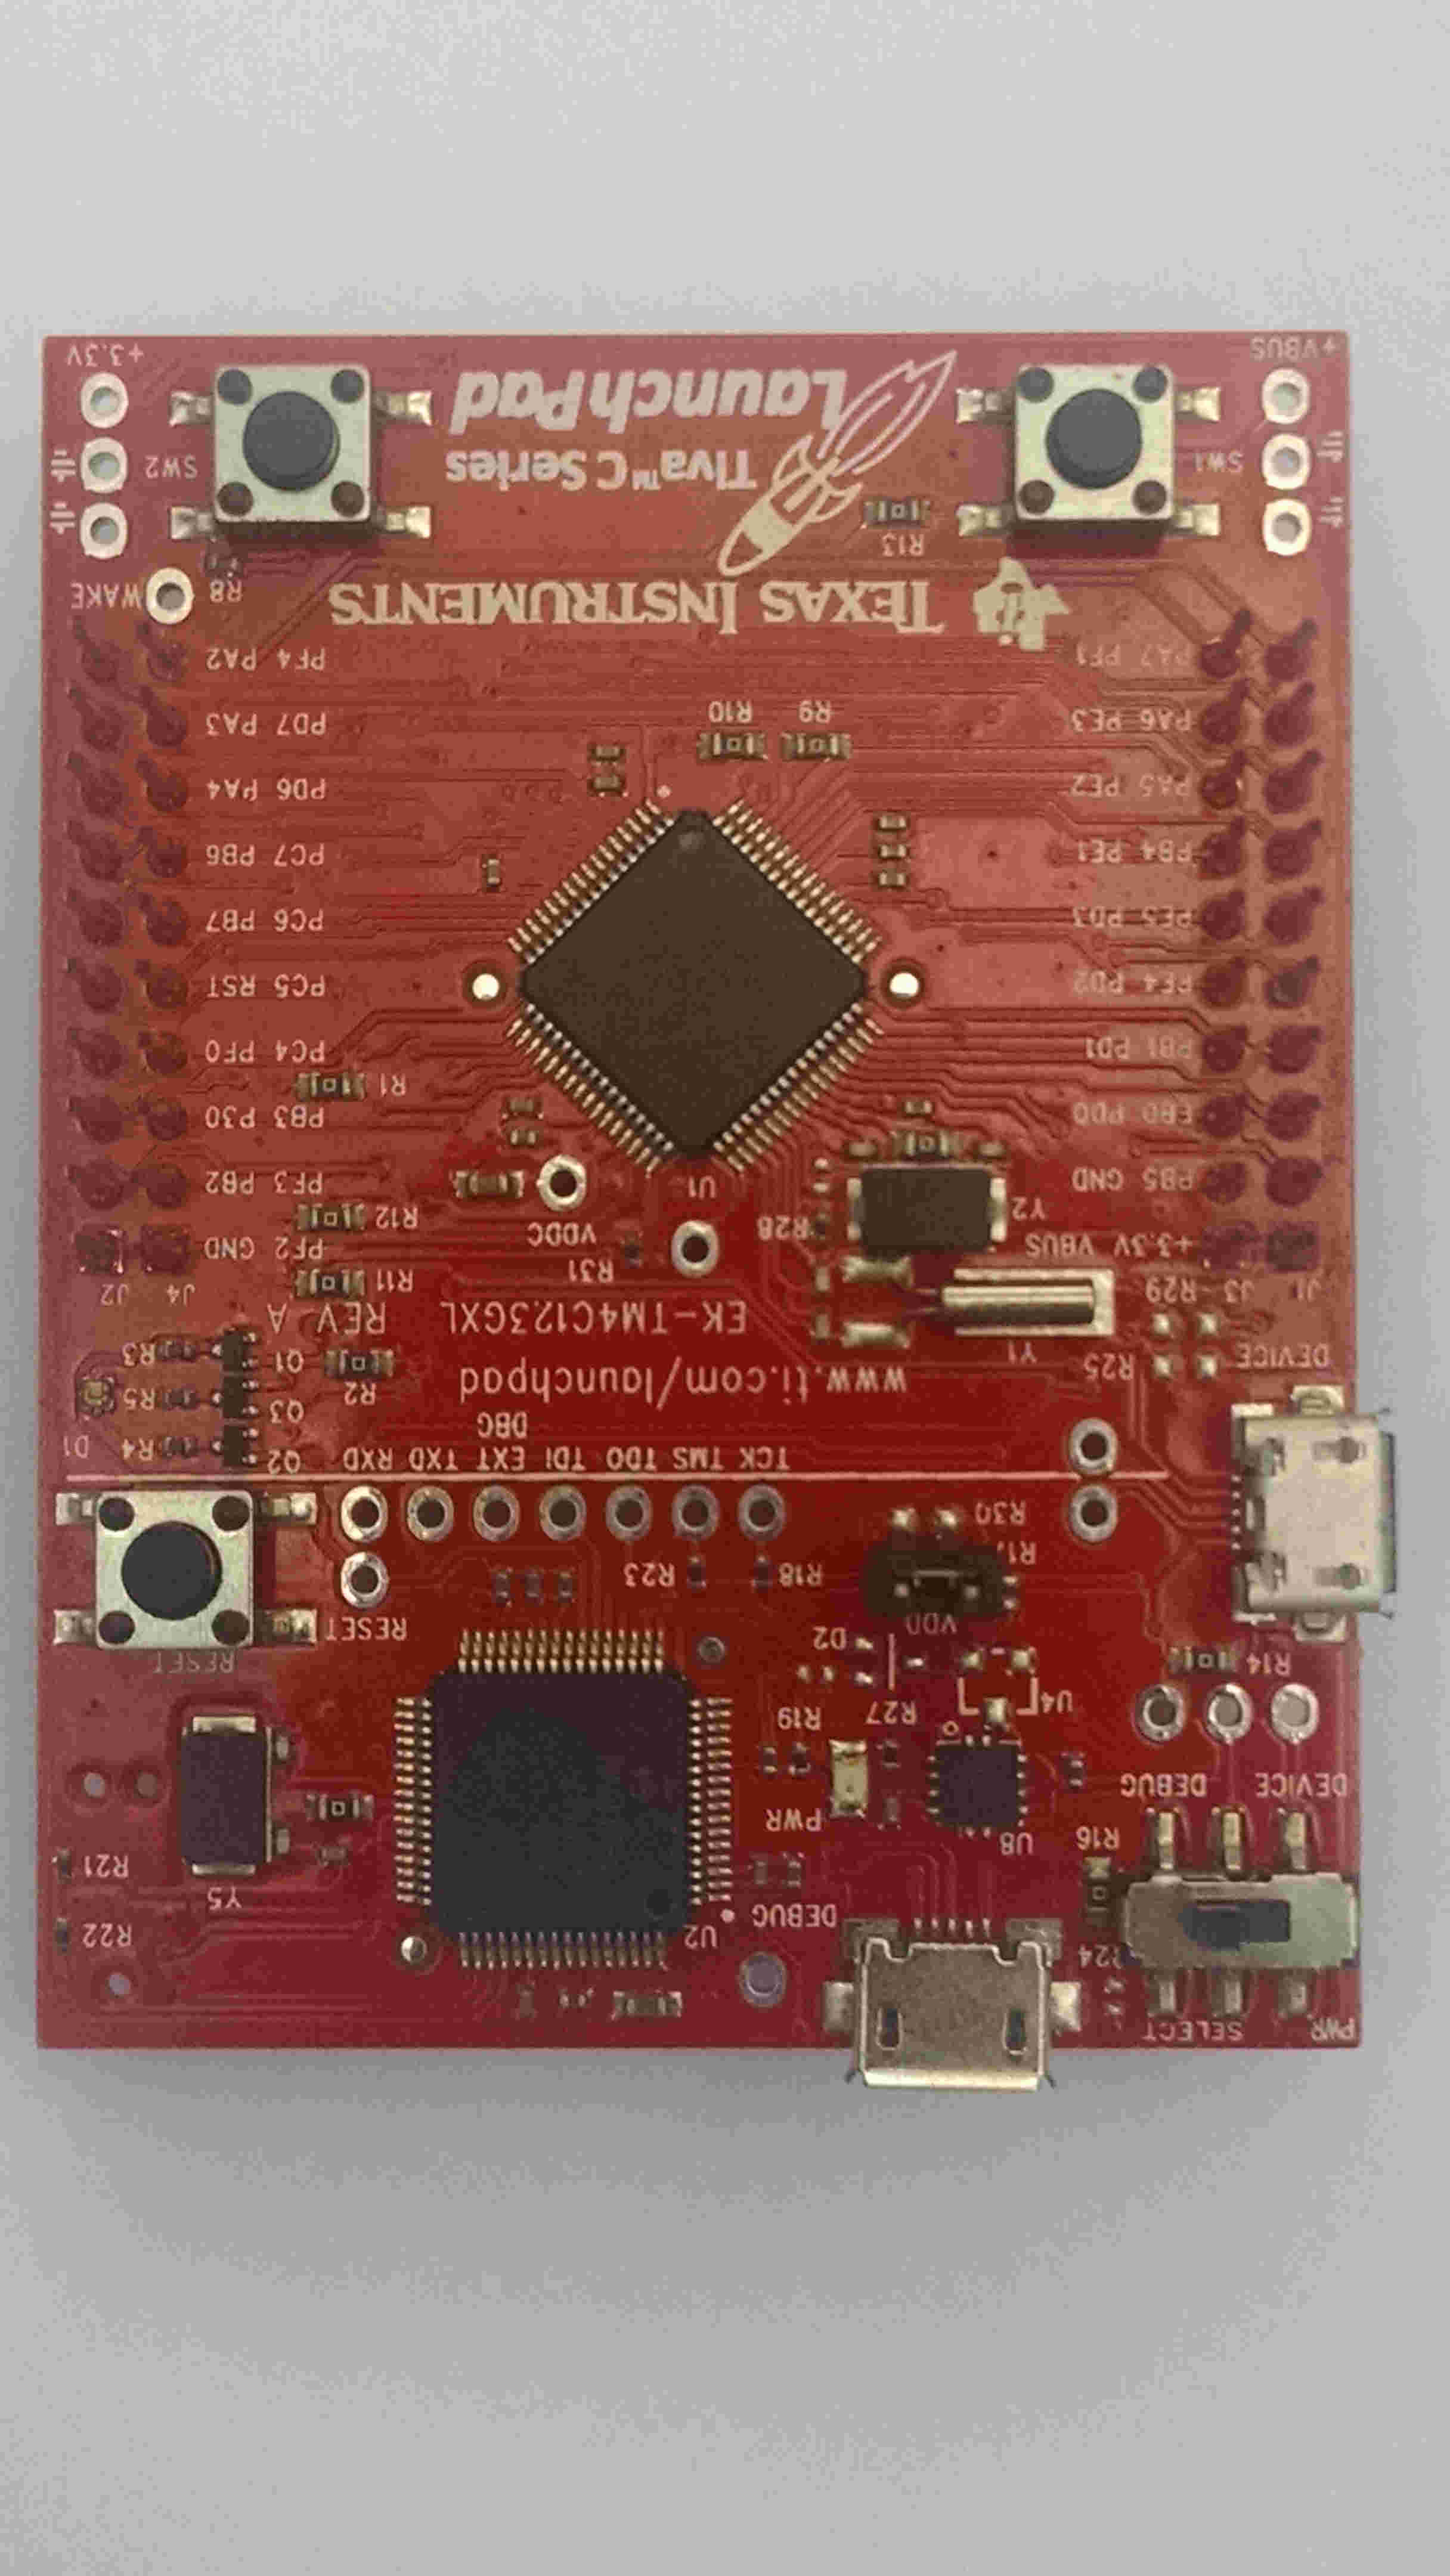
\includegraphics[scale=0.1, angle=180, clip=true, trim=0 750 60 500]{./imagens/uC-ARM.jpg}
%\caption{Microcontrolador}
%\label{fig:uCarm}
%\end{figure}


%\section{Programação}



%\begin{figure}[!htb]
%\centering
%\begin{tikzpicture}[scale=1]
%%\draw [lightgray](0,0) grid (16,10);

%\draw [black, thick](0,0) rectangle (16, 8); 
%\node at (1,7.7) {\textbf{\texttt{Sistema}}};


%\draw [black, thick](0.5,0.5) rectangle (7, 7); 
%\node at (0.9,6.7) {\textbf{\texttt{src}}};

%\node at (5,6) {main.c};
%\node at (2.5,5) {tm4c123gh6pm.h};
%\node at (5,4) {startup{\_}gcc.c};
%\node at (2,3) {linker.ld};
%\node at (2,2) {*.c};
%\node at (5,2) {*.h};



%\draw [black, thick](8,0.5) rectangle (15.5, 7); 
%\node at (9,6.7) {\textbf{\texttt{debug}}};

%\draw [black, thick](8.5,1) rectangle (15, 3); 
%\node at (9,2.7) {\textbf{\texttt{src}}};

%\node at (10,6) {\emph{Makefile}};

%\node at (10,5) {*.bin};
%\node at (13,5) {*.hex};
%\node at (10,4) {*.elf};
%\node at (13,4) {*.map};
 
%\node at (10,2) {*.d};
%\node at (13,2) {*.o};

%\end{tikzpicture}
%\caption{ Estrutura do Projeto}
%\label{fig:estruturaProjeto}
%\end{figure}




%\begin{figure}[!htb]
%\centering
%\begin{tikzpicture}[scale=1]
%\draw [lightgray](0,0) grid (16,10);

%\draw [black, ultra thick, dashed]( 0,8) rectangle ( 3,10); % terminal de comunicacao
%\node at (1.5,9.3){Terminal};
%\node at (1.5,8.7){Comunicação};
%\draw [ultra thick][->](1,8)--(1,4);
%\draw [ultra thick][->](2,4)--(2,8);

%\draw [black, ultra thick]( 0,2) rectangle ( 3, 4);  % serial
%\node at (1.5,3) {Serial};
%\draw [ultra thick][->](1.5,2) -- (1.5,1) -- (15,1) -- (15,2);

%\draw [black, ultra thick]( 5,2) rectangle ( 7, 4); % Fila
%\node at (6,3) {Fila};
%\draw [ultra thick][->](7,3)--(9,3);

%\draw [black, ultra thick]( 9,2) rectangle (12, 4); % Controlador
%\node at (10.5,3) {Controlador};
%\draw [ultra thick][->](12,3)--(14,3);

%\draw [black, ultra thick](14,2) rectangle (16, 4); % PWM
%\node at (15,3) {PWM};
%\draw [ultra thick][->](15.5,4)--(15.5,6);

%\draw [black, ultra thick]( 5,6) rectangle ( 7, 8); % Timer
%\node at (6,7) {Timer};
%\draw [ultra thick][->](6,6)--(6,4);
%\draw [ultra thick][->](5,6)--(3,4);
%\draw [ultra thick][<->](7,7)--(9,7);

%\draw [black, ultra thick]( 9,6) rectangle (12, 8); % Interrupt
%\node at (10.5,7) {Interrupt};
%\draw [ultra thick][->](11,6)--(11,4);
%\draw [ultra thick][->](10,6)--(7,4);

%\draw [black, ultra thick](14,6) rectangle (15,8); % In
%\node at (14.5,7) {In};
%\draw [ultra thick][->](14,7)--(12,7);
%\node at (14.3,9.5){Sensor};
%\draw [ultra thick][->](14.5,9)--(14.5,8);

%\draw [black, ultra thick](15,6) rectangle (16,8); % Out
%\node at (15.5,7) {Out};
%\draw [ultra thick][->](15.5,8)--(15.5,9);
%\node at (15.6,9.5){Drive};


%\end{tikzpicture}
%\caption{ Estrutura do Projeto}
%\label{fig:estruturaFirmware}
%\end{figure}




